%You can leave alone everything before Line 79.
\documentclass{article}
\usepackage{url,amsfonts, amsmath, amssymb, amsthm,color, enumerate}
 \usepackage{fullpage}
% Page layout
%\setlength{\textheight}{8.75in}
%\setlength{\columnsep}{2.0pc}
%\setlength{\textwidth}{6.5in}
%\setlength{\topmargin}{0in}
%\setlength{\headheight}{0.0in}
%\setlength{\headsep}{0.0in}
%\setlength{\oddsidemargin}{0in}
%\setlength{\evensidemargin}{0in}
%\setlength{\parindent}{1pc}
\newcommand{\shortbar}{\begin{center}\rule{5ex}{0.1pt}\end{center}}
\newcommand{\xxx}[1]{\textcolor{red}{#1}}
%\renewcommand{\baselinestretch}{1.1}
% Macros for course info
\newcommand{\courseNumber}{EECS 545}
\newcommand{\courseTitle}{Machine Learning}
\newcommand{\semester}{Winter 2012}
% Theorem-like structures are numbered within SECTION units
\theoremstyle{plain}
\newtheorem{theorem}{Theorem}[section]
\newtheorem{lemma}[theorem]{Lemma}
\newtheorem{corollary}[theorem]{Corollary}
\newtheorem{proposition}[theorem]{Proposition}
\newtheorem{statement}[theorem]{Statement}
\newtheorem{conjecture}[theorem]{Conjecture}
\newtheorem{fact}{Fact}
%definition style
\theoremstyle{definition}
\newtheorem{definition}[theorem]{Definition}
\newtheorem{example}{Example}
\newtheorem{problem}[theorem]{Problem}
\newtheorem{exercise}{Exercise}
\newtheorem{algorithm}{Algorithm}
%remark style
\theoremstyle{remark}
\newtheorem{remark}[theorem]{Remark}
\newtheorem{reduction}[theorem]{Reduction}
%\newtheorem{question}[theorem]{Question}
\newtheorem{question}{Question}
%\newtheorem{claim}[theorem]{Claim}
%
% Proof-making commands and environments
\newcommand{\beginproof}{\medskip\noindent{\bf Proof.~}}
\newcommand{\beginproofof}[1]{\medskip\noindent{\bf Proof of #1.~}}
\newcommand{\finishproof}{\hspace{0.2ex}\rule{1ex}{1ex}}
\newenvironment{solution}[1]{\medskip\noindent{\bf Problem #1.~}}{\shortbar}

%====header======
\newcommand{\solutions}[4]{
%\renewcommand{\thetheorem}{{#2}.\arabic{theorem}}
\vspace{-2ex}
\begin{center}
{\small  \courseNumber, \courseTitle
\hfill {\Large \bf {#1} }\\
\semester, University of Michigan, Ann Arbor \hfill
{\em Date: #3}}\\
\vspace{-1ex}
\hrulefill\\
\vspace{4ex}
{\normalsize Project Report}\\
{\LARGE  #2}\\
\vspace{2ex}
\end{center}
\begin{trivlist}
\item \textsc{Team members:} {#4}
\end{trivlist}
\noindent
\vspace{-1cm}
\shortbar
\vspace{-0.5cm}
}
% math macros
\newcommand{\defeq}{\stackrel{\textrm{def}}{=}}
\newcommand{\Prob}{\textrm{Prob}}
%==
\usepackage{graphicx}
\begin{document}
%%%%%%%%%%%%%%%%%%%%%%%%%%%%%%%%%%%%%%%%%%%%%%%%%
%\solutions{Your name}{Problem Set Number}{Date of preparation}{Collaborators}{Prover}{Verifiers}
\solutions{}{We need a title}{\today}{\\ Keegan R. Kinkade, @kinkadek\\ Pedro d'Aquino, @pdaquino \\Shiva Ghose, @gshiva }
%%%%%%%%%%%%%%%%%%%%%%%%%%%%%%%%%%%%%%%%%%%%%%%%%
%\renewcommand{\theproblem}{\arabic{problem}} 
%%%%%%%%%%%%%%%%%%%%%%%%%%%%%%%%%%%%%%%%%%%%%%%%%
%
% Begin the solution for each problem by
% \begin{solution}{Problem Number} and ends it with \end{solution}
%
% the solution for Problem 

\begin{abstract}

Robocode\cite{robocode} is a battle-tank simulator, for which players write robots in Java that compete among each other. Traditionally, most robots have been hand-coded. In this project, we create a robot that uses machine learning techniques to decide which actions to take. In particular, we use support vector machines to learn evasion and targeting strategies, with competitive results. We also implement Q-learning to learn targeting strategies, but with less success. We test our robot against some of the best Robocode robots available.
\end{abstract}

\section{Introduction}

Initially released in 2001 with the aim of assisting in learning object oriented programming, Robocode is an open source, dynamic, deterministic tank battling simulator implemented in Java. Each Robocode agent is designed with the ability to control a robotic tank, including a differentially-driven movement platform, a $360\,^{\circ}\mathrm{}$ rotating turret and an enemy scanning radar, in order to attempt to destroy other tanks with similar features but opposing strategies. While the environment has made creating a simple working agent capable of moving, targeting, and shooting easy, perfecting agents to do well against multiple opponent strategies has proven to be difficult. There has been research to optimize agents using both neural networks as well as genetic programming. However, little work has been done to incorporate sophisticated machine learning techniques designed to better inform Robocode agents when making decisions inside the battle environment.

\subsection*{Statement of the Problem}

\xxx{Explain more about how Robocode works}

The purpose of this project is to incorporate machine learning algorithms in a Robocode agent in order to optimize the agent's ability to stay alive during battles. Specifically, we focus on incorporating machine learning in two areas: \emph{evasion} and \emph{targeting}. To simplify the models, we consider these areas separately.

With respect to evasion, our goal is to evade incoming bullets in order to maximize the expected lifetime of the agent. For targeting, the goal is to maximize the accuracy of the bullets our robot fires.

We create agents that learn good strategies for both areas, and then create one robot that combines the learned evasion and targeting strategies. We then measure its performance by competing against human-written robots and evaluating the score of the battle, which is computed by Robocode based on damage inflicted and number of victories.

\xxx{This probably should go in the next section (it was in the previous paragraph):}

 we gather environmental information on employing multiple missile evasion strategies against different opponents in an effort to determine which evasive strategy to employ given a specific situation to ultimately reduce the likelihood of being struck by an opponent's missile.  Furthermore, we used machine learning algorithms in order to predict how an opponent will react upon learning that our agent has fired, thus allowing our agent to take advantage of the ability to predict opponent's behavior. Such an application of machine learning within multi-agent games provides the framework and motivation to explore different techniques in designing artificial agents capable of making perceptually informed decisions on how to best interact with their environment. 

%\section{Experimental Approach}
%
%Movement and Targeting were treated as two independent functions. This assumption is valid because we can decouple the actions of the gun and the movement platform. The task of evasion was implemented as a subset of strategies which the agent chooses to employ. Targeting was implement in two different approaches: the first was similar to evasion in that an agent had subset of actions to choose from, the second method explored the use of reinforcement learning.
%
%%Building a Robocode agent equipped with machine learning algorithms to better inform its decision making will be broken into two unique tasks: evasion and targeting. Each task will have a subset of strategies which the agent can choose to employ in order to evade or target an opponent. In order to decide which strategy to employ for a given task, the agent will make use of machine learning techniques to analyze the current situation within the environment and choose the strategy which maximizes the likelihood of achieving the task goal. 
%
%\subsection*{Movement Strategy}
%
%%Within the task of evasion, there are two movement approaches that need to be considered:
%%\begin{itemize}
%
%%\item General movement 
%
%%\item Evasive movement 
%%\end{itemize}
%
%%Each approach to movement needs to be employed based on the situation,  and the agent will need to learn which evasive movement strategy %to employ when engaged in the general movement strategy.
%
%\subsubsection*{General Movement }
%In general the probability of getting hit by incoming fire is inversely proportional to how close the observer is to the firing point. We wanted our agent to move closer to the enemy when it had higher health to maximize the probability of hitting the enemy and stay further back when it had lower health to better evade incoming fire. This was modeled as series of attracting and repelling force interactions. The general movement of the agent was to mirror the opponent at a fixed distance in order to avoid collisions with the enemy while better assessing the effectiveness of the evasion strategies. 
%
%\subsubsection*{Evasive Movement }
%%Every time an agent fires a bullet, their energy drops proportionally to the speed of the bullet they fired. Built into Robocode is the ability to detect the energy drop of an opponent, and thus agents are capable of detecting when an enemy has fired a bullet. From such an energy drop, agents can determine the location a bullet was fired, and the velocity of the bullet, but not the direction with which the enemy fired in.
%Our agent constantly monitors the actions taken by the opponent and upon detecting that the enemy has fired a bullet, it chooses an evasion strategy to employ. In order to do so, we began by creating a subset of relatively trivial evasion strategies and ran the differing evasion strategies when fired upon in multiple training battles against different opponents. Each time an evasion strategy was employed, we captured features in the environment as well as whether or not the strategy was effective in evading the bullet. We then trained support vector machines (SVMs) for each of the different evasion strategies using the features collected. After training, the agent can \emph{query} the SVMs and choose the best strategy corresponding to the SVM which produces the largest margin for evading the bullet. 
%
%\subsection*{Offensive Strategy}
%The offensive strategy deals with modeling where the opponent will be if the agent were to fire at a given point of time under a given set of environmental conditions. Simple movement vector extrapolations will fail against all but the most rudimentary opponents as they tend to employ advanced evasive strategies upon being fired at. Hence a more sophisticated prediction scheme is required to allow the agent to successfully target and attack the opponent. To this end we employed two methods: an SVM based approach and a Reinforcement Learning (RL) approach. 
%
%\subsubsection*{SVM Targeting}
%Using SVMs was similar to the evasive strategy where the agent uses the learnt the utilities of a set of strategies.
%
%\subsubsection*{RL Targeting}
%
%The RL strategy on the other hand involved slowly training the agent to handle more and more complicated evasion strategies.\\
%
%
% We finally compared the differences in using SVMs and RL methods for this kind of application.

%To this end, we plan on building up a probabilistic distribution of the opponents evasive reactions over time in order to better predict where to fire bullets. Furthermore, using training data in a similar fashion to that proposed in the evasion section, we will use an additional support vector machine to determine what situations lead to maximum likelihood of hitting the enemy when firing a bullet. This will ensure we only attempt to shoot at an enemy when we have a good chance of hitting them, thus reducing the amount of energy lost from making bad firing decisions. 
 
\section{Review of Related Work}
%We have found some articles describing genetic programming approaches to Robocode, but none that combines it with reinforcement learning. Eisenstein, in 2003, was the first to use genetic programming in this context \cite{gp2}. He found that, while he was able to beat some hand coded adversaries, his robots had a hard time learning how to target, and were therefore more likely to try to ram their opponents.\\

Robocode was introduced to teach Java as an object oriented programming language. However it also provides a powerful base upon which artificial intelligence methods can built up, taught and tested. This aspect of Robocode was explored as early as 2004 by Hartness \cite{Hartness}. Over the years various approaches have been used to develop highly competitive robots in this platform. The most successful so far have been systems built up on hand tuned heuristics which are aided by statistical methods. The majority of the research work done in this environment has been towards the application of Genetic Algorithms in evolving agents rather than evolving strategies \cite{strategies, gp1, gp2}.  Shichel et al. \cite{gp1}, used genetic programming to evolve tank strategies for a robot in the HaikuBot category (which allows robots whose code is no longer than 4 lines). They evolved a population of 256 robots over approximately 400 generations. Their robot was ranked 3rd in the HaikuBot category. Woolley et al. \cite{woolley} discuss the implementation of a hybrid reactive robot control system and use Robocode as a platform to verify their claims. Their work focuses on the ability of their system to mimic existing reactive control architectures. Reinforcement learning has also been used in Robocode to develop movement strategies for agents\cite{gade}. Other researchers have looked into using Neuro-Evolutionary methods with Augmented Topologies (NEAT) and Artificial Neural Networks (ANNs) \cite{nielsenAI} to control the targeting systems.\\

In one of the very few academic mentions of Robocode outside of the artificial intelligence field, Kobayashi et al. make a study of various sets of targeting strategies employed in Robocode \cite{strategies}. However they do not explicitly state any methods to calculate the expected utilities of employing each strategy given a scenario.\\

%The majority of the successful agents documented within Robocode arena employ sophisticated hand tuned methods when evading bullets and targeting their opponent. Many of the advanced agents employ varying forms of the k-means algorithm to cluster similar environmental situations and learn from these situations. However, most of the actual firing of bullets and evading incoming rounds is not done using sophisticated, statistical algorithms. \\

%Thus, our work will not only build upon the current ability to learn when to take certain actions in the environment, but also learn how to best carry out actions. 

The work we present in this paper presents a novel implementation of a combination of Support Vector Machines and Reinforcement Learning methods to design an agent which is capable of competing with the top most agents in Robocode.

\section{Experimental Methodology}
Movement and Targeting were treated as two independent functions. This assumption is valid because we can decouple the actions of the gun and the movement platform. The task of evasion was implemented as a subset of strategies which the agent chooses to employ. Targeting was implement in two different approaches: the first was similar to evasion in that an agent had subset of actions to choose from, the second method explored the use of reinforcement learning.

\subsubsection*{General Movement}
The default behavior of the agent is to closely mimic the behavior of the opponent while maintaining a set distance from it. The force of attraction/repulsion between the agent and its opponent is given by:
$$\emph{Force} = k_1 * (\emph{Distance to Opponent} - d)$$
where $k_1$ is a proportional factor while $d$ is the distance to maintain from the opponent. Thus if the agent is further away from the opponent than desired, it will experience an attractive force $+_{ve}F$ which will move it towards the opponent. Conversely, if the agent is to close to the opponent, it will experience a repulsive force $-_{ve}F$, which will guide it away. It is also evident that \emph{Force} becomes zero as \emph{Distance to Opponent}  $\rightarrow d$.\\ 

\begin{figure}[h]
	\centering
		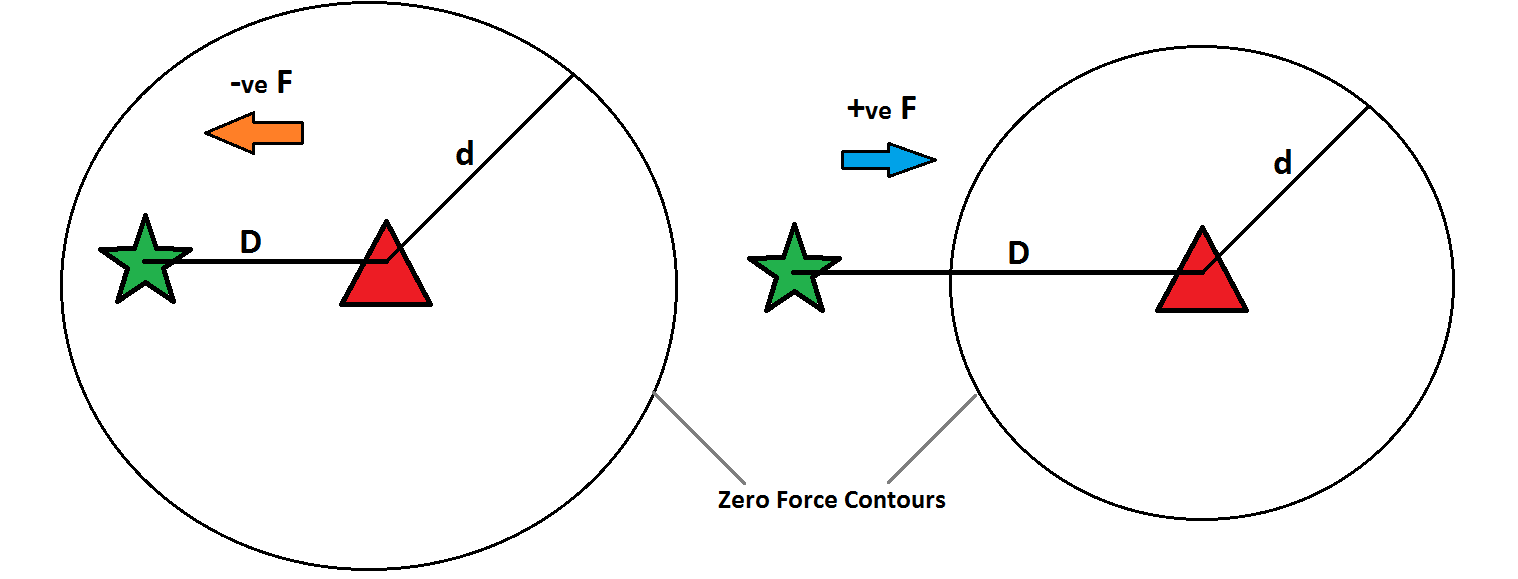
\includegraphics[width= 10cm]{mirror}
		\caption{The agent (represented by the green star) will attempt to move to the zero-potential force contour around the opponent (represented by the red triangle). This is not a strict mirroring of the opponent, but rather allows the agent to move to optimal positions as opposed to just being guided by the opponent.}		
	\label{mirror}
\end{figure}

When the agent's health is higher, it moves closer to the opponent in order to maximize offensive capabilities. Else, the agent will move further away from the enemy to reduce the chance of being shot. $d$ is a function of the agent's health and the opponent's health which is determined as:
$$d = d_{const} - k_2*(\emph{Health}_{Agent} - \emph{Health}_{Opponent})$$
where $d_{const}$ is the minimum distance to maintain from the opponent, and $k_2$ provides regularization on how much to depend on the health difference.

%In general, the closer a tank is to the opponent, the higher the probability that it will hit the target. Thus, in order to improve the odds of our agent's firing solution, we would like the agent to be near the opponent. However, when trying to avoid being hit by incoming fire, we would like to be far from the opponent. In order to find a compromise we modeled $d$ as a function of the agent's health and the opponent's health. When the agent's health is higher, it moves closer to the opponent in order to maximize offensive capabilities. Else, the agent will move further away from the enemy to reduce the chance of being shot. Hence, the value of $d$ is determined as:
%$$d = d_{const} - k_2*(\emph{Health}_{Agent} - \emph{Health}_{Opponent})$$
%where $d_{const}$ is the minimum distance to maintain from the opponent, and $k_2$ provides regularization on how much to depend on the health difference.

\subsection*{Evasion Strategies}
When the opponent fires at the agent, the mirroring behavior is suppressed and an evasion strategy is chosen. For training, we designed the system to choose a random strategy so that the agent has the ability to explore the entire state space and not form a biased opinion early on, thereby limiting itself. Given enough training points, we feel that the SVM is be able to find a good decision boundary with which to determine successful dodging strategies based on environmental properties. 

\subsubsection*{Dodge Left/Right}
In this strategy, the agent moves to the left or right of the opponent when it is fired upon. This movement strategy is represented in Figure \ref{LR}, where $\Psi$ is the relative bearing to the opponent ($-180^{\circ} \leq \Psi \leq 180^{\circ}$). There are two different turning cases for $\Psi$: one when the agent is facing direction $d_1$ corresponding to bearing $\Psi_1$, and second when the agent is facing direction $d_2$ corresponding to bearing $\Psi_2$. Because we have a differential driven robot, we desire to turn a minimum distance to position our drive track perpendicular to the line of sight between us and the opponent. Achieving this angle is done in tandem with moving either forward or backward depending on whether we are dodging left or right. Dodging left / right are implemented separately, giving the agent the ability to choose each strategy.\\

\begin{figure}[h]
\begin{minipage}[b]{0.5\linewidth}
	\centering
		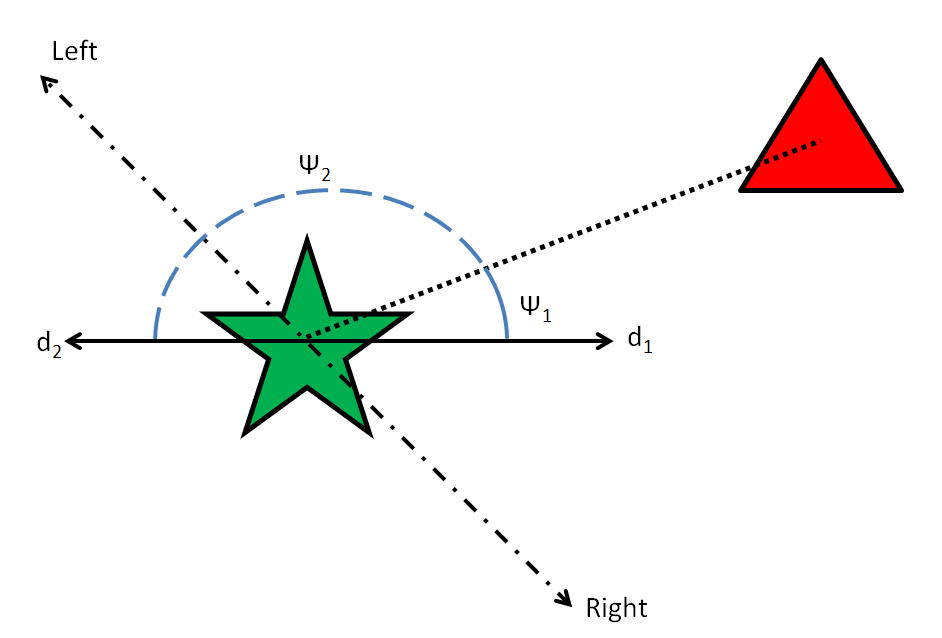
\includegraphics[width=6 cm]{LR}
	\caption{Left--Right dodging strategy. \emph{Note -- in Robocode, the angles are positive in a clockwise direction}}
	\label{LR}
\end{minipage}
\hspace{0.5cm}
\begin{minipage}[b]{0.5\linewidth}
	\centering
		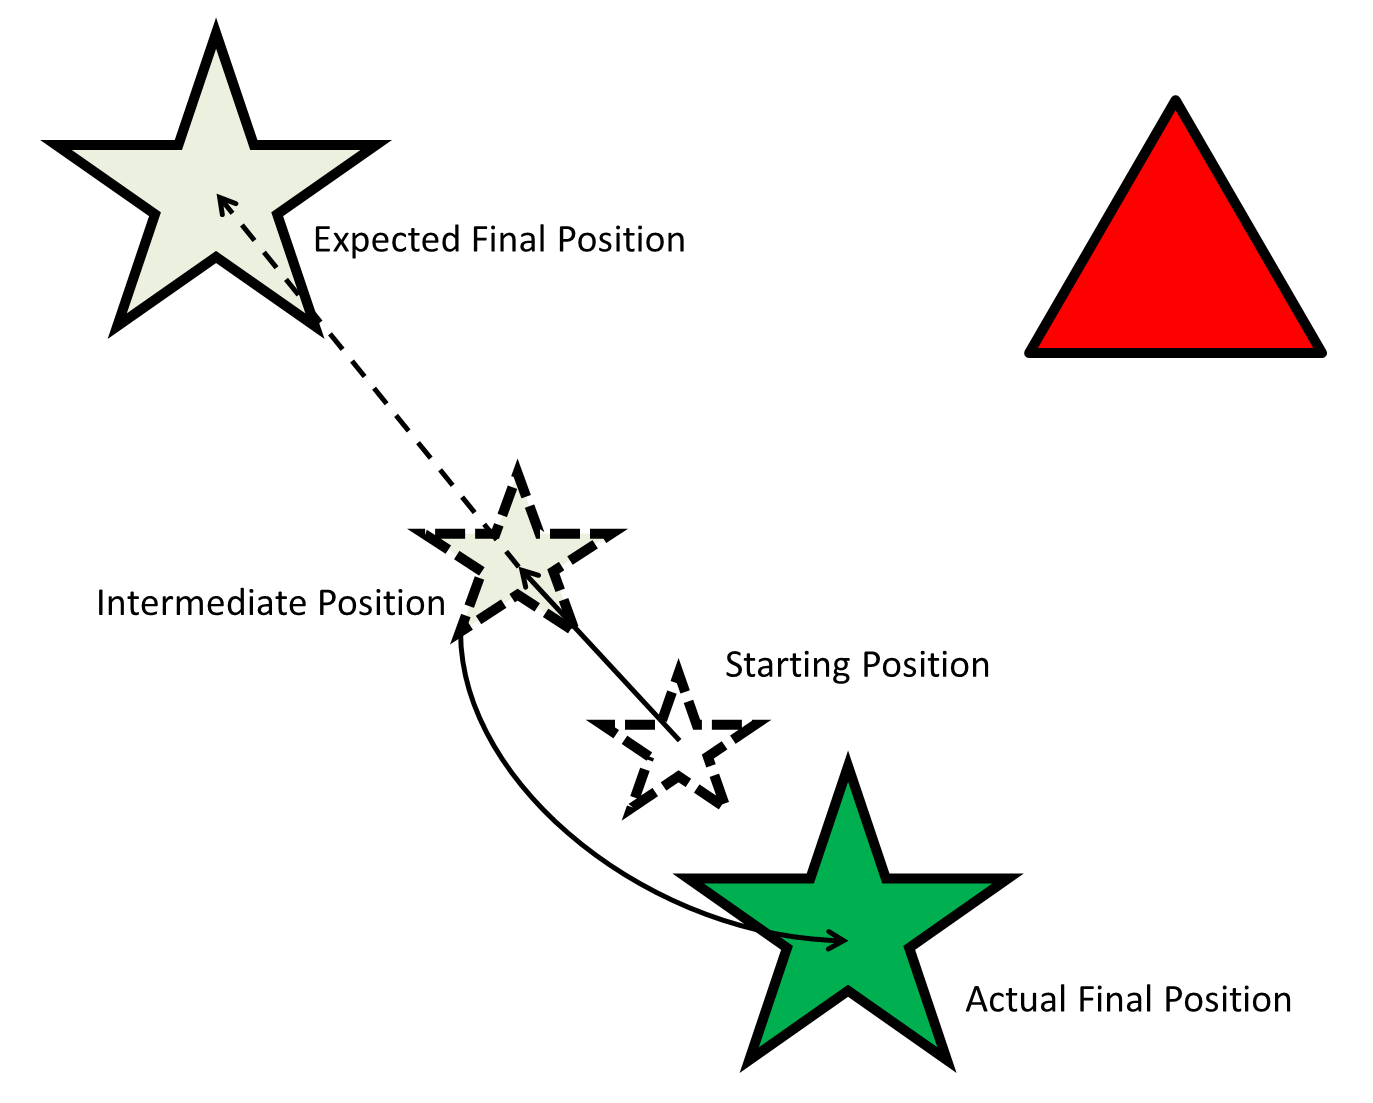
\includegraphics[width=6 cm]{Feign.png}
	\caption{Feigning}
	\label{feign}
\end{minipage}
\end{figure}

\subsubsection*{Feign}
In this strategy, upon detecting incoming fire, the agent immediately reverses its direction of motion. It can be seen in figure \ref{feign}.


%Robocode physics will require the agent to slow down to a stand still and then accelerate in the new direction.
%It is evident to us that this strategy will fail at closer distances and if the agent is moving directly towards or away from the opponent. Thus we expect the SVMs to discern this over time and only apply feign when it is optimal to do so.


\subsubsection*{Random Movement}
%Random movement is useful against opponents that try to model their opponents.
For this strategy, we set the turn control and forward movement control to a random value chosen from a uniform distribution. Agents that move in such a random manner are said to have flat movement profiles. They are hard to target, but certain advanced opponents are programmed to monitor such movement strategies when the agent approaches a wall or a corner, in which case the very nature of the environment will cause a spike in their movement profile.

\subsection*{Evaluation of Movement Strategies}
With these strategies created, we needed a way to check the effectiveness of a evasion scheme. At its essence, we were testing the ability of the agent to stay alive, but we cannot rely on survival time alone as a measure of the effectiveness of a strategy. Thus, the effectiveness of the strategies are tested by the ability of the agent to dodge a particular shot fired at it. This is done through an estimate of the shot which is implemented using \emph{Bullet Tracking}.

\subsubsection*{Bullet Tracking}
In order to determine if the evasion strategy employed was effective in dodging the bullet that was fired at the agent, we devised a way to track the bullet. In Robocode this is not a straight forward task, as the agent cannot sense a bullet using its radar. However, in order to fire a bullet, a tank must sacrifice some of its own energy. The radar-sensor can detect a drop in energy of the opponent, and using this we can determine if the enemy has fired a bullet as well as the bullet's velocity. This is given by the formula:
$$\emph{Bullet Velocity} = 20 - 3 * \emph{Energy Drop}$$
Using the velocity coupled with some basic Newtonian Physics\footnote{$\emph{Distance} = \emph{Velocity} * \emph{Time}$}, we can predict all the possible positions the bullet can be at a given time step.
%The contours will be circular while resembling the motion of a wave. Hence, these estimates are known as \emph{waves}.
Figure \ref{b_wave} illustrates this wave pattern taken on by bullets. Our objective is to see if we get hit by a bullet when the projected wave hits us, in which case we register a failure of the dodge strategy. Otherwise, we can conclude that we have successfully dodged the bullet.

\begin{figure}[h]
\begin{minipage}[b]{0.5\linewidth}
	\centering
		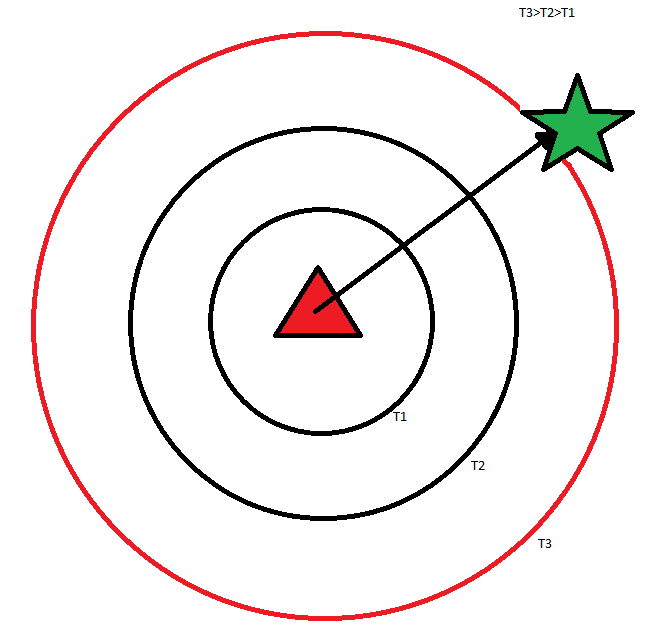
\includegraphics[width=5 cm]{bullet_wave.png}
	\caption{Bullet waves at different time steps}
	\label{b_wave}
\end{minipage}
\hspace{0.5cm}
\begin{minipage}[b]{0.5\linewidth}
\centering
		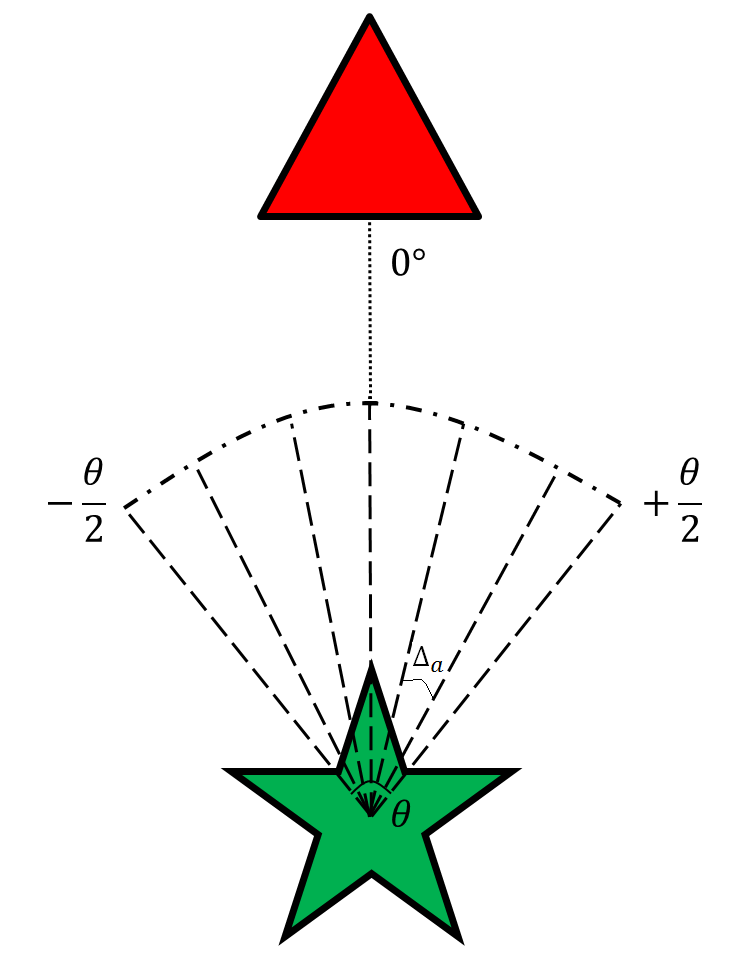
\includegraphics[width=5 cm]{targeting.png}
	\caption{Discretization of targeting solutions}
	\label{tget}
\end{minipage}
\end{figure}

\subsection*{Targeting Strategies}
The approach taken for targeting was completely different from the movement strategy. Instead of providing a set of targeting strategies based on heuristics such as linear movement targeting, circular movement targeting, etc. we chose to let our machine learning methods learn optimal targeting schemes from scratch. The objective of a targeting agent is to predict where the opponent will be in the future and shoot accordingly. The statespace for the targeting agent to act in is virtually infinite $[0^{\circ}, 360^{\circ}]$ , so in order make calculations tractable, we discretized the operating region as demonstrated in figure \ref{tget}. For both the SVM targeting scheme and the RL targeting scheme, we allowed the agent to choose one of 21 possible firing angles which were evenly distributed between $[-\frac{\theta}{2}, +\frac{\theta}{2}]$, where $\theta$ is the firing arc range and $0^{\circ}$ represents head on alignment with the opponent.


%We are currently at a point where we can begin to collect data for evasive maneuvering. During the course of the training, we will look at the effectiveness of each strategy as the ability to dodge a particular shot while ignoring any other bullets which hit us during our evasive maneuver. We will collect data by running each evasion strategy multiple times against multiple different agents. 



\subsubsection*{SVMs}

\xxx{TODO}

\subsubsection*{Q-learning}
Q-learning \cite{watkins92a} learns a $Q(s, a)$ function that attributes an utility value to taking an action $a$ at state $s$. This method
has two interesting properties. First, it doesn't require a model of the environment. This is desirable because modelling the
interactions between our robot, its opponent and the environment would be overly complex and time consuming. Second, the $Q$ function
takes into account future states. For instance, it might be the case that
at a certain state $s_0$, firing at the opponent will likely miss, but will make it move to a state with much higher utility. In this scenario,
firing might be the optimal action even though the likelihood of hitting the opponent is low. It is impossible to learn this using our
SVM-based approach, because it cares only about the current state.

More specifically, we use a linear approximation for the $Q(s, a)$ function:

$$Q(s, a) = w_a^T\phi(s)$$

where $w_a$ is a weight vector associated with that action, and $\phi(s)$ is the feature vector that encodes the current state.\\

We could have alternatively modeled the function as $Q(s,a) = w^T\phi(s, a)$. This would have increased the learning rate because only
one weight vector would be necessary. However, designing $\phi(s, a)$ is very challenging.

In principle, there are infinite possible actions (all possible firing angles between $-180^{\circ} $ and $180^{\circ} $ -- we consider $0^{\circ}$ to be straight at the opponent),
so we need to discretize the
action space. Because we use a different weight vector for every action, it is desirable to minimize the number of actions in order
to increase the learning rate. After some preliminary testing, we decided to limit the firing angle to $[-40^{\circ}, 40^{\circ}]$ ($\theta = 80^{\circ}$), and to uniformly discretize this arch into
21 actions, each separated by $\Delta_a = 3.8^{\circ}$, this is demonstrated in figure \ref{tget}.

To handle situations where the optimal firing angle is not exactly one of the 21 actions, we add randomness: when we choose to fire at angle $a_i$, we uniformly sample the actual
firing angle between $a_i - \Delta_a/2$ and $a_i + \Delta_a/2$. In this case, the robot may happen to sample the optimal firing angle. Given enough training examples, it will
eventually learn that choosing $a_i$ has the possibility of hitting the opponent. However, it makes learning harder and slower.

Reinforcement learning problems generally deal with exploration/exploitation tradeoffs. In order to have more predictable and comparable results, we decided to
create one robot for exploration, and one for exploitation. This is akin to training/testing in other machine learning problems.

During training, we randomly choose an action $a_i$ and employ it. To evaluate its effectiveness, we need to know $s'$, the new state after we fire,
and $R(s, a_i)$, the reward we obtained. We record $s'$ after $t$ have passed since firing. This captures information on
how the opponent tried to evade the bullet (remember that the opponent is able to detect it has been fired upon, but is unable to know where the bullet is).
The value of the reward $R(s, a_i)$ is discovered once the robot is notified the bullet hit or missed. We then apply the learning equation \cite{russelnorvig}:

$$w_a = w_a + \alpha\left[R(s, a_i) + \gamma\max_{a'}Q(s', a') - Q(s, a_i)\right]\phi(s)$$

After the weights have been updated, we fire again.\\

We test using a greedy policy subject that fires at the angle with the highest $Q$ value. If the highest value at a certain state is below a threshold, then
the agent does not fire.

\section{Results}
\xxx{Short Intro?}

\subsection*{Evasion Results}
\xxx{TODO}

\subsection*{Targeting Results}
\xxx{TODO}

\subsubsection*{SVM Targeting}
\xxx{TODO}

\subsubsection*{RL Targeting}
\xxx{TODO}

\subsection*{Integrated Performance}
\xxx{TODO}

\section{Conclusion}

\xxx{TODO}

%Thus far, we have successfully written an agent capable of implementing the previously discussed evasion techniques when fired upon by an opposing agent. This agent is also capable of continuously tracking the enemy, as well as the bullets fired from the enemy, in an effort to capture the data needed to train each evasion strategy's SVM. We are currently in the process of choosing the exact features desired from the environment upon each evasion attempt, and will then begin collecting data with which to train the SVMs on. After such training, we will then be able to evaluate the evasion system in an effort to maximize the agent's ability to evade bullets as well as to capture those features most important to understanding the best strategy given each unique situation. Lastly, we will move onto repeating these steps, with the additional knowledge gained throughout our experience, to design an effective targeting and firing system. At the end of this project, we will have novelly employed machine learning techniques to artificial intelligence agents in order to improve their ability to make decision informed by their perceptual knowledge of the environment.

\bibliographystyle{IEEEtranS}
\bibliography{sources}

\end{document}


\def\therefore{\boldsymbol{\text{ }
\leavevmode
\lower0.4ex\hbox{$\cdot$}
\kern-.5em\raise0.7ex\hbox{$\cdot$}
\kern-0.55em\lower0.4ex\hbox{$\cdot$}
\thinspace\text{ }}}
